\chapter{SAF microarchitecture design space}

This section summarizes key design choices which form the SAF microarchitecture design space.

\section{SAF attributes}
%
% Figure: SAF attributes impact uarch cost
%
\begin{figure*}[ht]
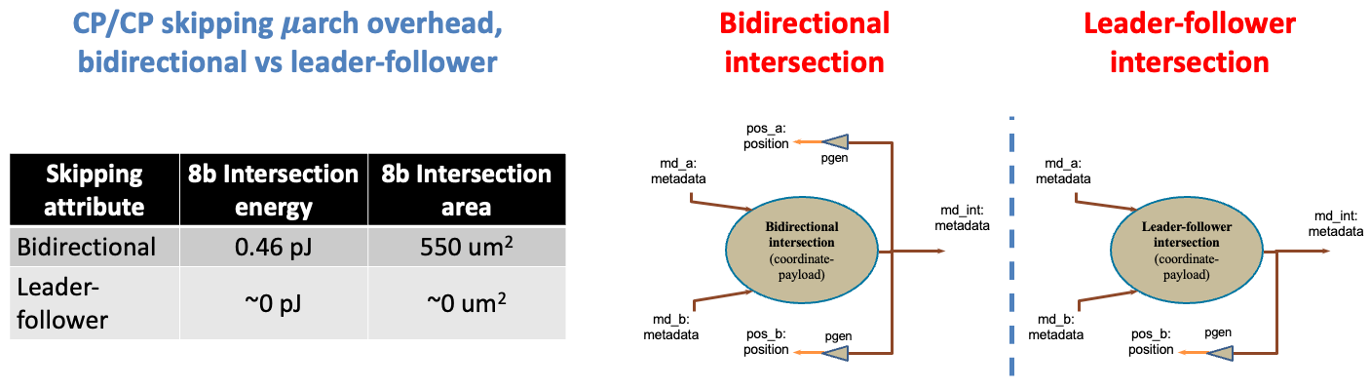
\includegraphics[width=\textwidth]{figures/saf_attributes_impact_uarch_cost.PNG}
\caption{Zero-skipping microarchitecture cost-comparison between an architecture with a bidirectional skipping SAF (left) and an architecture with a leader-follower skipping SAF (right.) Both architectures also employ a coordinate-payload format SAF.}
\label{fig:saf_attributes_impact_uarch_cost}
\centering
\end{figure*}
%
% Content: SAF attributes impact SAF microarchitecture cost
%
The attributes of a SAF impact the energy, area and latency of its SAF microarchitecture by implicitly constraining aspects of the design-space.
%
\subsection{SAF microarchitecture topology and primitive cost} 

Figure \ref{fig:saf_attributes_impact_uarch_cost} shows that a skipping SAF with the leader-follower attribute can have an implementation based on simple control logic that conditions MACs and follower reads on whether there is a nonzero leader operand. The energy and area overhead to implement this SAF is low. However designers may choose bidirectional skipping SAF instead in order to skip 100\% of ineffectual operations; this results in more expensive skipping microarchitecture with comparison logic to detect either or both zero operands, incurring a significant energy and area overhead. Generally, simple changes in the SAF optimization strategy may (or may not) have dramatic impact on microarchitecture complexity and thus on energy, area and latency.
%
\subsection{SAF primitive design}
%
\todo{Don't use terminology (i.e. primitive) which is not yet introduced.}
%
\section{Load-handling requirements}
%
\section{Optimizations}

\subsection{Algorithm}

\subsection{Pipelining}
%
\section{Cross-architecture impacts}

